\documentclass[11pt,letterpaper]{article}

\usepackage[margin=1in]{geometry}
\usepackage{amsmath,amssymb}
\usepackage{graphicx}
\usepackage{array}
\usepackage[round]{natbib}

\setlength{\parskip}{0.4em}
\setlength{\parindent}{1.5em}
\setlength{\emergencystretch}{1.5em}
\renewcommand{\arraystretch}{1.22}

\title{\textbf{Breaking the Moratorium Trap: Emergent Cultivation--Depensation Bistability and Ecosystem-Based Recovery of Northwest Atlantic Cod (\emph{Gadus morhua})}}

\author{
  Quantitative Marine Ecosystem Modelling Group\\[0.3em]
  \small Prepared for submission to the \emph{Canadian Journal of Fisheries and Aquatic Sciences}\\[0.2em]
  \small Running head: \emph{Cultivation--Depensation and Atlantic Cod Recovery}
}

\date{}

\begin{document}
\maketitle

\begin{abstract}
\noindent
Following catastrophic groundfish overexploitation across the Northwest Atlantic shelf in the late twentieth century, Canada imposed an indefinite commercial fishing moratorium on Atlantic cod (\emph{Gadus morhua}) in July 1992. More than three decades later, cod spawning stock biomass (SSB) across major shelf divisions remains below 2\%--5\% of historical benchmarks despite near-zero directed fishing mortality. Single-species stock--recruitment theory predicts rapid demographic rebuilding once fishing mortality falls below intrinsic replacement, leaving persistent non-recovery an enduring paradox in fisheries science. Here we construct and calibrate a dynamic six-species, physiologically structured size-spectrum model of the Northwest Atlantic shelf community---comprising capelin (\emph{Mallotus villosus}), Atlantic herring (\emph{Clupea harengus}), Atlantic mackerel (\emph{Scomber scombrus}), shorthorn/longhorn sculpins (\emph{Myoxocephalus} spp.), American plaice (\emph{Hippoglossoides platessoides}), and Atlantic cod---implemented in the R package \texttt{mizer}. Using identical biological, bioenergetic, and trophic interaction parameters, linear stability analysis of the continuous-time McKendrick--von Foerster Jacobian reveals two coexisting asymptotically stable equilibria at zero cod fishing ($F_{\mathrm{cod}} = 0\text{ yr}^{-1}$): a cultivated, cod-dominated state ($\mathrm{SSB}_{\mathrm{cod}} = 1018.2\text{ kt}$, leading eigenvalue $\max\operatorname{Re}(\lambda) = -0.1809\text{ yr}^{-1}$) and a collapsed, forage-locked moratorium state ($\mathrm{SSB}_{\mathrm{cod}} = 15.8\text{ kt}$, $\max\operatorname{Re}(\lambda) = -0.0084\text{ yr}^{-1}$) sustained only by sheltered inshore coastal refuges. When overfishing pushes cod past a saddle-node fold bifurcation at $F_{\mathrm{cod}}^{*} \approx 0.250\text{ yr}^{-1}$, release from adult cod predation triggers a $5.4$-fold biomass surge across pelagic forage fishes and benthic sculpins. This guild reversal elevates instantaneous predation mortality on $0.05$--$5\text{ g}$ larval and $0$-group cod from $0.25\text{ yr}^{-1}$ (cultivated) and $0.69\text{ yr}^{-1}$ (sustainable fishery) to $7.33\text{ yr}^{-1}$ while depressing juvenile feeding levels via shared zooplankton depletion. Equilibrium continuation scans and $40$-year policy projections demonstrate that while status-quo moratoria remain trapped indefinitely below the $29.5\text{ kt}$ separatrix, a time-limited $20$-year harvest pulse on abundant pelagic planktivores ($F_{\mathrm{pelagic}} = 0.65\text{ yr}^{-1}$) and sculpins ($F_{\mathrm{mesopred}} = 0.45\text{ yr}^{-1}$) breaks the early-life predation bottleneck, restores adult cod top-down control, and supports a self-sustaining reopened cod fishery ($F_{\mathrm{cod}} = 0.15\text{ yr}^{-1}$) after forage harvest returns to baseline.

\vspace{0.5em}
\noindent\textbf{Keywords:} Atlantic cod (\emph{Gadus morhua}), cultivation--depensation, alternative stable states, hysteresis, size-spectrum modelling, \texttt{mizer}, ecosystem-based fisheries management, forage fish.
\end{abstract}

\section{Introduction}

The 1992 collapse of Northwest Atlantic cod (\emph{Gadus morhua}) off Newfoundland and Labrador, in the Gulf of St.~Lawrence, and on the eastern Scotian Shelf represents one of the most consequential ecological and socio-economic transformations in modern marine history \citep{hutchings1994what,myers1997why,lilly2013review}. Driven by decades of escalating distant-water and domestic otter-trawl exploitation that pushed instantaneous fishing mortality well above sustainable thresholds, spawning stock biomass (SSB) declined by more than 98\% from mid-twentieth-century levels \citep{hutchings1994what,myers1997why}. When the Government of Canada declared a commercial moratorium in July 1992, standard single-species surplus-production and age-structured stock assessment models projected recovery to harvestable biomass within roughly one to two cod generations (8--15 years), assuming compensatory Beverton--Holt or Ricker recruitment at low spawner density. Instead, more than three decades after directed trawling ceased, major offshore stock complexes remain locked at 1\%--5\% of historical spawner abundance, persisted largely via localized inshore fjord aggregations such as Smith Sound in Trinity Bay \citep{shelton2006fishing,swain2008predicted,lilly2013review}.

Multiple hypotheses have been advanced to explain this prolonged non-recovery, including elevated natural mortality of adult cod from pinniped predation and metabolic stress \citep{swain2008predicted,shelton2006fishing}, fisheries-induced life-history shifts, bycatch in reopened inshore or invertebrate fisheries, and community-wide trophic reorganization \citep{frank2005trophic,bundy2005can}. Empirical syntheses from the eastern Scotian Shelf, southern Gulf of St.~Lawrence, and Grand Banks point compellingly to a dramatic restructuring of shelf food webs following apex groundfish removal \citep{swain2000pelagic,frank2005trophic}. Specifically, the collapse of large-bodied piscivorous cod released small pelagic planktivores---notably Atlantic herring (\emph{Clupea harengus}), Atlantic mackerel (\emph{Scomber scombrus}), and capelin (\emph{Mallotus villosus})---alongside benthic mesopredators such as shorthorn and longhorn sculpins (\emph{Myoxocephalus} spp.), whose combined biomasses expanded several-fold during the 1990s and 2000s \citep{frank2005trophic,bundy2005can}. In the southern Gulf of St.~Lawrence, \citet{swain2000pelagic} documented a strong negative relationship between pelagic herring and mackerel biomass and cod recruitment rate per unit SSB, consistent with intense consumption of pelagic cod eggs and larvae by filter- and particulate-feeding clupeids and scombrids.

\citet{walters2001cultivation} formalized this mechanism conceptually as the \emph{cultivation--depensation} hypothesis: in size-structured aquatic food webs, large adult piscivores ``cultivate'' favourable nursery conditions for their own offspring by cropping down smaller-bodied forage fishes and mesopredators that would otherwise prey upon or compete with piscivore eggs, larvae, and newly settled juveniles. If overfishing depletes adult piscivores below a critical threshold, released forage and mesopredator populations surge and impose a severe early-life demographic bottleneck---an emergent Allee effect (depensation) that prevents piscivore recovery even after directed fishing is eliminated completely ($F = 0$). Subsequent theoretical studies using stage-structured biomass models \citep{vanleeuwen2008how,gardmark2015regime} showed that ontogenetic diet shifts and size-dependent predation can generate alternative stable states, while empirical analyses on the Scotian Shelf suggested that transient signs of groundfish recovery only emerged when bloated forage fish stocks began outstripping their own zooplankton food supply \citep{frank2011transient}.

Despite its central policy relevance, translating cultivation--depensation from conceptual two-species stage models to operational fisheries advice requires resolving continuous body-size structure across multiple interacting guild members, realistic fleet size-selectivity, and explicit bioenergetic feedback between plankton depletion, somatic growth, and size-selective mortality \citep{andersen2010damped,scott2014mizer,andersen2019fish}. In continuous multi-species size-spectrum models, cohort survival from egg weight $w_0$ to maturation weight $w_{\mathrm{mat}}$ is governed by the cumulative physiological mortality integral
\begin{equation}
  S(w_0 \to w_{\mathrm{mat}}) = \exp\!\left(-\int_{w_0}^{w_{\mathrm{mat}}} \frac{\mu(w)}{g(w)}\,\mathrm{d}w\right),
  \label{eq:survival}
\end{equation}
where $\mu(w)$ is total instantaneous mortality and $g(w)$ is somatic growth rate \citep{andersen2019fish}. Equation~\eqref{eq:survival} reveals a potent \emph{dual trophic squeeze} during forage outbreaks: abundant planktivores and benthic mesopredators simultaneously inflate $\mu(w)$ via direct predation on $1\text{ mg}$--$15\text{ g}$ cod and depress $g(w)$ by grazing down shared zooplankton prey, lengthening the duration juvenile cod remain vulnerable within the ``predator pit''.

In this paper, we develop and calibrate a six-species Northwest Atlantic shelf size-spectrum model in \texttt{mizer} \citep{scott2014mizer,delius2022mizer} to address three questions: (1) Can empirically grounded life-history, size-selection, and trophic-overlap parameters generate rigorous, asymptotically stable cultivation--depensation bistability at $F_{\mathrm{cod}} = 0$? (2) Why has a 34-year cod moratorium failed to restore cod dominance, and where do the saddle-node collapse and recovery tipping points lie? (3) Can targeted, time-limited ecosystem harvest of overabundant forage and mesopredator guilds reverse the trophic lock and transition the ecosystem permanently back to a self-sustaining cod fishery without chronic forage depletion? To bridge quantitative size-spectrum theory and fisheries governance, we also pair our analysis with an interactive web-based policy simulator designed for fisheries managers and stakeholders.

\section{Materials and Methods}

\subsection{Continuous Multi-Species Size-Spectrum Framework}

We model the shelf fish community using the continuous-time, size-structured McKendrick--von Foerster conservation PDE framework implemented in \texttt{mizer} version 3.4 \citep{scott2014mizer,andersen2019fish}. For each fish species $i \in \{1,\dots,6\}$, the number density $N_i(w,t)$ ($\text{individuals}\cdot\text{g}^{-1}$) at individual body mass $w \in [w_0, w_{\infty,i}]$ evolves according to
\begin{equation}
  \frac{\partial N_i(w,t)}{\partial t} + \frac{\partial \big[g_i(w,t)\,N_i(w,t)\big]}{\partial w} = -\mu_i(w,t)\,N_i(w,t),
  \label{eq:mvf}
\end{equation}
coupled to a lower-trophic plankton/benthos resource spectrum $N_R(w,t)$ spanning $w \in [w_{\min,R}, w_{\mathrm{cut},R}]$ governed by semichemostat dynamics at each size bin:
\begin{equation}
  \frac{\partial N_R(w,t)}{\partial t} = r_R(w)\,\big[c_R(w) - N_R(w,t)\big] - \mu_{p,R}(w,t)\,N_R(w,t),
  \label{eq:resource}
\end{equation}
with carrying capacity $c_R(w) = \kappa w^{-\lambda}$ ($\kappa = 2.8 \times 10^{11}\text{ g}^{\lambda-1}$, spectral slope $\lambda = 2.08$, cutoff $w_{\mathrm{cut},R} = 10\text{ g}$) and weight-invariant turnover rate $r_R = 10\text{ yr}^{-1}$ across a logarithmic grid of $100$ consumer size bins from $w_0 = 1\text{ mg}$ to $15\text{ kg}$.

Predators encounter prey according to a lognormal size-selection kernel
\begin{equation}
  \phi_i(w, w_p) = \exp\!\left[-\frac{\big(\ln(w / (w_p \beta_i))\big)^2}{2\sigma_i^2}\right],
  \label{eq:kernel}
\end{equation}
parameterized by preferred predator--prey mass ratio $\beta_i$ and diet breadth $\sigma_i$. Total food encounter rate for a predator of species $i$ and mass $w$ is
\begin{equation}
  E_i(w,t) = \gamma_i w^{q_i} \int \phi_i(w, w_p)\,\left[N_R(w_p,t) + \sum_{j=1}^{6} \theta_{ij}\,N_j(w_p,t)\right] w_p\,\mathrm{d}w_p,
  \label{eq:encounter}
\end{equation}
where $\gamma_i w^{q_i}$ is volumetric search rate ($q_i = 0.8$) and $\theta_{ij} \in [0,1]$ is the dimensionless spatial and vertical habitat overlap matrix between predator $i$ and prey $j$. Feeding level follows a Holling Type II functional response $f_i(w,t) = E_i(w,t) / [E_i(w,t) + h_i w^{n_i}]$ with maximum intake $h_i w^{n_i}$ ($n_i = 0.75$). Assimilated energy $\alpha_{\mathrm{assim}} f_i(w,t) h_i w^{n_i}$ ($\alpha_{\mathrm{assim}} = 0.6$), net of standard metabolic maintenance $k_{s,i} w^{p_i}$ ($p_i = 0.75$), is partitioned via maturity ogive $\psi_i(w)$ between somatic growth $g_i(w,t)$ and reproductive investment $E_{\mathrm{repro},i}(w,t)$ \citep{scott2014mizer,andersen2019fish}.

Conversely, predation mortality inflicted on prey $j$ of mass $w_p$ integrates over all larger piscivores and planktivores whose feeding kernels span $w_p$:
\begin{equation}
  \mu_{p,j}(w_p,t) = \sum_{i=1}^{6} \theta_{ij} \int \phi_i(w, w_p)\,\big(1 - f_i(w,t)\big)\,\gamma_i w^{q_i}\,N_i(w,t)\,\mathrm{d}w,
  \label{eq:predmort}
\end{equation}
and total mortality is $\mu_j(w,t) = \mu_{0,j}(w) + \mu_{p,j}(w,t) + F_j(w,t)$, where $\mu_{0,j}(w) = z_{0,j} (w / w_{\infty,j})^{n_j - 1}$ captures non-modelled predation by marine mammals, seabirds, large pelagics, and physiological senescence, and $F_j(w,t)$ is size-selective fishing mortality.

\subsection{Northwest Atlantic Community Parameterization and Inshore Refuges}

We represent the Northwest Atlantic continental shelf community through six functional species spanning four trophic roles (Table~\ref{tab:species}):
\begin{enumerate}
  \item \textbf{Boreal and temperate pelagic planktivores:} Capelin (\emph{Mallotus villosus}, $w_\infty = 50\text{ g}$), Atlantic herring (\emph{Clupea harengus}, $w_\infty = 380\text{ g}$), and Atlantic mackerel (\emph{Scomber scombrus}, $w_\infty = 850\text{ g}$). High preferred predator--prey mass ratios ($\beta = 2000, 2500, 350$) and broad feeding kernels ($\sigma = 1.8$--$2.2$) reflect particulate and filter feeding on copepods, euphausiids, and pelagic fish eggs and larvae ($1\text{ mg}$--$2\text{ g}$).
  \item \textbf{Benthic ambush mesopredator:} Sculpin guild (\emph{Myoxocephalus scorpius} and \emph{M.~octodecemspinosus}, $w_\infty = 1100\text{ g}$, $\beta = 65$, $\sigma = 1.6$), representing demersal cottids that surged across Newfoundland and Scotian Shelf grounds post-1992 and prey heavily upon newly settled $0$-group and age-$1$ demersal cod ($0.5$--$25\text{ g}$).
  \item \textbf{Benthic flatfish competitor:} American plaice (\emph{Hippoglossoides platessoides}, $w_\infty = 2600\text{ g}$, $\beta = 220$), a benthivorous flatfish sharing invertebrate/small-fish prey without strong ichthyoplankton predation on cod.
  \item \textbf{Apex ontogenetic omnivore/piscivore:} Atlantic cod (\emph{Gadus morhua}, $w_\infty = 15\,000\text{ g}$, $w_{\mathrm{mat}} = 850\text{ g}$, $\beta = 60$, $\sigma = 1.6$), which hatches at $w_0 = 1\text{ mg}$, feeds on plankton below $10$--$20\text{ g}$, transitions onto capelin, juvenile clupeids, and benthic invertebrates at intermediate sizes, and exerts strong top-down predation on adult capelin, herring, mackerel, and sculpins above $1\text{ kg}$.
\end{enumerate}

\begin{table}[t!]
\centering
\caption{Life-history, feeding-kernel, calibration biomass, and recruitment parameters for the six-species Northwest Atlantic shelf size-spectrum model. Observed calibration biomasses $B_{\mathrm{obs}}$ ($1\text{ kt} = 10^9\text{ g}$) apply above survey selectivity cutoff $w_{\mathrm{cut}}$ at the reference exploitation state ($F_{\mathrm{cod}} = 0.22\text{ yr}^{-1}$). Reproductive efficiencies $\varepsilon_{\mathrm{repro}}$ emerge from steady-state calibration.}
\label{tab:species}
\vspace{0.4em}
\resizebox{\textwidth}{!}{%
\begin{tabular}{lrrrrrrrrrr}
\hline
Species & $w_\infty$ (g) & $w_{\mathrm{mat}}$ (g) & $k_{\mathrm{vb}}$ ($\text{yr}^{-1}$) & $z_0$ ($\text{yr}^{-1}$) & $\beta$ & $\sigma$ & $B_{\mathrm{obs}}$ (kt) & $w_{\mathrm{cut}}$ (g) & $r_{\mathrm{level}}$ & $\varepsilon_{\mathrm{repro}}$ \\
\hline
Capelin   &    50 &   7 & 0.75 & 0.38 & 2000 & 1.8 & 520 &  2 & 0.88 & $1.70 \times 10^{-3}$ \\
Herring   &   380 &  55 & 0.58 & 0.35 & 2500 & 2.2 & 380 & 10 & 0.88 & $5.72 \times 10^{-4}$ \\
Mackerel  &   850 & 115 & 0.52 & 0.34 &  350 & 1.9 & 190 & 15 & 0.88 & $2.27 \times 10^{-4}$ \\
Sculpin   &  1100 &  95 & 0.42 & 0.54 &   65 & 1.6 & 140 & 15 & 0.88 & $4.81 \times 10^{-4}$ \\
Plaice    &  2600 & 180 & 0.28 & 0.28 &  220 & 1.7 & 260 & 20 & 0.88 & $7.36 \times 10^{-5}$ \\
Cod       & 15000 & 850 & 0.26 & 0.20 &   60 & 1.6 & 680 & 50 & 0.28 & $2.12 \times 10^{-6}$ \\
\hline
\end{tabular}%
}
\end{table}

The trophic interaction matrix $\theta_{ij}$ (Table~\ref{tab:inter}) encodes ontogenetic role reversal on the shelf. Adult cod overlap strongly with capelin ($\theta_{\mathrm{Cod,Cap}} = 0.45$), herring ($0.43$), mackerel ($0.40$), and sculpin ($0.38$), whereas spawning/feeding aggregations of herring ($\theta_{\mathrm{Her,Cod}} = 1.00$), mackerel ($\theta_{\mathrm{Mac,Cod}} = 1.00$), and capelin ($\theta_{\mathrm{Cap,Cod}} = 0.55$) overlap intensely with buoyant pelagic cod eggs and larvae in surface waters \citep{swain2000pelagic}, and demersal sculpins ($\theta_{\mathrm{Scu,Cod}} = 0.45$) overlap with newly settled $0$-group cod on coastal and bank nurseries. Note that $\theta_{ij}$ weights only spatial/habitat co-occurrence; actual predation strictly obeys the predator--prey mass kernel $\phi_i(w, w_p)$ in eq.~\eqref{eq:kernel}, so a $250\text{ g}$ herring ($\beta = 2500$) preys solely upon $\sim 0.01$--$1\text{ g}$ larval cod and cannot consume juvenile or adult cod.

\begin{table}[t!]
\centering
\caption{Dimensionless trophic habitat-overlap matrix $\theta_{ij}$ (rows = predators $i$, columns = prey $j$) governing realized encounter rates alongside the size-selection kernel $\phi_i(w, w_p)$.}
\label{tab:inter}
\vspace{0.4em}
{\small
\setlength{\tabcolsep}{7pt}
\begin{tabular}{lrrrrrr}
\hline
Predator $\backslash$ Prey & Capelin & Herring & Mackerel & Sculpin & Plaice & Cod \\
\hline
Capelin   & 0.01 & 0.01 & 0.01 & 0.01 & 0.01 & 0.55 \\
Herring   & 0.02 & 0.01 & 0.01 & 0.01 & 0.02 & 1.00 \\
Mackerel  & 0.04 & 0.02 & 0.01 & 0.01 & 0.02 & 1.00 \\
Sculpin   & 0.05 & 0.02 & 0.01 & 0.02 & 0.03 & 0.45 \\
Plaice    & 0.04 & 0.02 & 0.01 & 0.01 & 0.01 & 0.02 \\
Cod       & 0.45 & 0.43 & 0.40 & 0.38 & 0.12 & 0.025 \\
\hline
\end{tabular}
}
\end{table}

Boundary recruitment at $w_0$ combines standard offshore Beverton--Holt density dependence with a small coastal refuge flux $R_{\mathrm{refuge},i}$:
\begin{equation}
  R_{\mathrm{dd},i}(t) = \frac{R_{\mathrm{di},i}(t)}{1 + R_{\mathrm{di},i}(t) / R_{\max,i}} + R_{\mathrm{refuge},i}, \qquad
  R_{\mathrm{di},i}(t) = \frac{\varepsilon_{\mathrm{repro},i}}{2 w_0} \int_{w_0}^{w_{\infty,i}} E_{\mathrm{repro},i}(w,t)\,N_i(w,t)\,\mathrm{d}w,
  \label{eq:rdd}
\end{equation}
installed via \texttt{setRateFunction(params, "RDD", "RefugeBevertonHoltRDD")}. Following empirical observations that post-1992 Northern and Gulf cod persisted in sheltered inshore fjords (such as Smith Sound, Trinity Bay, and Gilbert Bay) largely decoupled from offshore clupeid/scombrid predation \citep{lilly2013review}, we set $R_{\mathrm{refuge,Cod}}$ to $1.1\%$ of calibrated reference cod recruitment ($R_{\mathrm{refuge},i} = 0$ for all other species). Because eq.~\eqref{eq:rdd} is smooth ($C^\infty$) everywhere, all steady-state and Jacobian eigenvalue operators remain exact.

Four size-selective commercial fleets operate with logistic length-based selectivity curves (\texttt{sigmoid\_\allowbreak length}, parameterized by 50\% and 25\% retention lengths $L_{50}$ and $L_{25}$; Table~\ref{tab:gears}): (1) a \texttt{Pelagic} purse-seine/midwater trawl fleet harvesting capelin ($L_{50} = 11\text{ cm}$, catchability $q = 0.75$), herring ($L_{50} = 20\text{ cm}$, $q = 1.0$), and mackerel ($L_{50} = 25\text{ cm}$, $q = 1.0$); (2) a \texttt{Mesopredator} coastal pot/trap fleet targeting adult sculpins ($L_{50} = 20\text{ cm}$, $q = 1.0$) with negligible cod bycatch; (3) a \texttt{Flatfish} fleet targeting American plaice ($L_{50} = 28\text{ cm}$, $q = 1.0$); and (4) a directed \texttt{Cod\_Trawl} groundfish fleet targeting adult cod ($L_{50} = 52\text{ cm}$, $L_{25} = 45\text{ cm}$, $q = 1.0$).

\begin{table}[t!]
\centering
\caption{Commercial fishing fleets, target species, logistic length-selectivity parameters ($L_{50}, L_{25}$), catchabilities, and baseline pre-collapse/moratorium fishing efforts.}
\label{tab:gears}
\vspace{0.4em}
\resizebox{\textwidth}{!}{%
\begin{tabular}{llrrrrr}
\hline
Fleet / Gear & Species & $L_{50}$ (cm) & $L_{25}$ (cm) & Catchability $q$ & Pre-Collapse $F$ ($\text{yr}^{-1}$) & Moratorium $F$ ($\text{yr}^{-1}$) \\
\hline
Pelagic      & Capelin  & 11 &  9 & 0.75 & 0.15 & 0.15 \\
Pelagic      & Herring  & 20 & 16 & 1.00 & 0.15 & 0.15 \\
Pelagic      & Mackerel & 25 & 20 & 1.00 & 0.15 & 0.15 \\
Mesopredator & Sculpin  & 20 & 16 & 1.00 & 0.05 & 0.05 \\
Flatfish     & Plaice   & 28 & 23 & 1.00 & 0.15 & 0.15 \\
Cod\_Trawl   & Cod      & 52 & 45 & 1.00 & 0.15 & 0.00 \\
\hline
\end{tabular}%
}
\end{table}

\subsection{Calibration, Linear Stability Analysis, and Scenario Experiments}

Model calibration proceeded iteratively at a moderate exploitation reference ($F_{\mathrm{cod}} = 0.22\text{ yr}^{-1}$, $F_{\mathrm{pelagic}} = 0.15\text{ yr}^{-1}$, $F_{\mathrm{mesopred}} = 0.05\text{ yr}^{-1}$, $F_{\mathrm{flatfish}} = 0.15\text{ yr}^{-1}$) by alternating \texttt{matchGrowth()}, \texttt{matchBiomasses()}, \texttt{steadySingleSpecies(..., keep = "biomass")}, \texttt{setBevertonHolt()}, and \texttt{tuneSteadyState()} until observed biomasses, von Bertalanffy growth rates, and size spectra converged simultaneously to machine accuracy with physiologically realistic reproductive efficiencies ($\varepsilon_{\mathrm{repro},i} \in [2.12 \times 10^{-6}, 1.70 \times 10^{-3}] \ll 1$; Table~\ref{tab:species}). Imposing Beverton--Holt dimensionless reproduction levels $r_{\mathrm{level}} = R_{\mathrm{dd}} / R_{\max}$ ($0.88$ for prey guilds, reflecting strong recruitment compensation when released from predation, and $0.28$ for cod) together with $R_{\mathrm{refuge,Cod}}$ yielded the final parameter object.

Holding all biological, interaction, gear, and resource parameters strictly fixed, we located steady states via \texttt{findSteadyState()} (requiring relative rate-of-change residuals $< 10^{-5}\text{ yr}^{-1}$ and confirming \texttt{isSteady()}) and assessed local asymptotic stability by computing the full $826 \times 826$ continuous-time ODE Jacobian spectrum (600 consumer bins plus 226 resource bins) via \texttt{getStability()} \citep{delius2022mizer}. Equilibrium hysteresis branches were traced via pseudo-continuation (\texttt{scanModel(..., continuation = TRUE)}) forward and backward across $F_{\mathrm{cod}} \in [0, 0.50]\text{ yr}^{-1}$ and $F_{\mathrm{pelagic}} \in [0, 0.70]\text{ yr}^{-1}$ (at $F_{\mathrm{cod}} = 0$). Finally, we simulated the 61-year historical trajectory from 1965 to 2026---sustainable groundfish fishing ($F_{\mathrm{cod}} = 0.15\text{ yr}^{-1}$, 1965--1967), distant-water trawling expansion ($F_{\mathrm{cod}} = 0.46\text{ yr}^{-1}$, 1968--1980), acute pre-collapse overfishing ($F_{\mathrm{cod}} = 0.56\text{ yr}^{-1}$, 1981--1991), and the 34-year commercial moratorium ($F_{\mathrm{cod}} = 0.00\text{ yr}^{-1}$, 1992--2026)---followed by six 40-year management scenarios from 2026 to 2066 alongside a $7 \times 6 \times 6 \times 2$ policy response grid exported to our interactive web simulator (\texttt{docs/index.html}).

\section{Results}

\subsection{Historical Collapse, Guild Reversal, and the Post-1992 Moratorium Trap}

Starting from the sustainable pre-collapse fishery equilibrium in 1965 ($\mathrm{SSB}_{\mathrm{cod}} = 776.3\text{ kt}$, cod landings $129\text{ kt}\cdot\text{yr}^{-1}$), simulated escalation of directed otter-trawl effort during 1968--1991 reproduces the trajectory and trophic cascade observed across Northwest Atlantic shelf divisions (Fig.~\ref{fig:history}). As adult cod biomass is eroded past the cultivation threshold during the 1980s, cod SSB plunges by $99.3\%$ to $5.7\text{ kt}$ in 1992 (Fig.~\ref{fig:history}A). Concurrently, predation release triggers an explosive community-wide guild reversal: combined adult biomass of capelin, herring, mackerel, and sculpins surges more than five-fold, reorganizing the shelf from a piscivore-controlled demersal system into a planktivore- and mesopredator-dominated state.

\begin{figure}[t!]
  \centering
  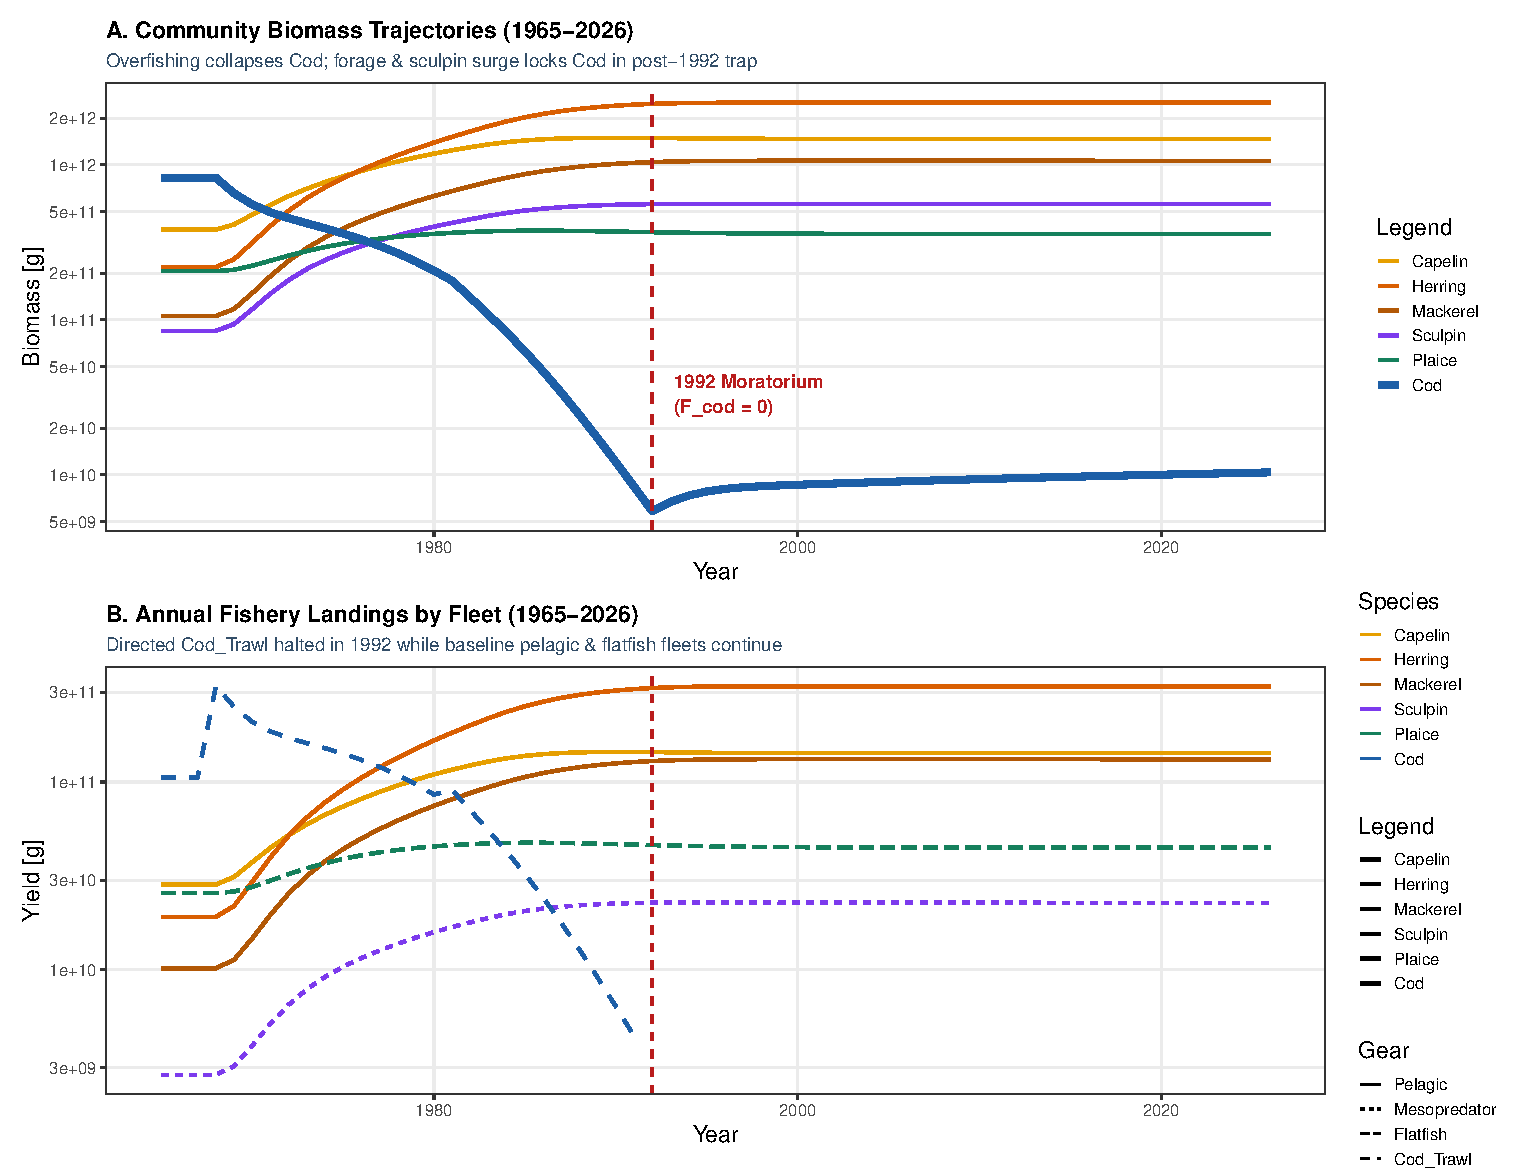
\includegraphics[width=0.95\textwidth]{figures/fig1_collapse_moratorium.pdf}
  \caption{Simulated historical groundfish collapse (1965--1992) and post-moratorium trophic lock (1992--2026). \textbf{(A)} Biomass trajectories of the six shelf species above survey cutoffs (\texttt{plotBiomass}), highlighting Atlantic cod. Escalating trawl effort ($F_{\mathrm{cod}} = 0.46 \to 0.56\text{ yr}^{-1}$) collapses cod by $>99\%$ by 1992 and releases a multi-species surge of herring, capelin, mackerel, and sculpin. \textbf{(B)} Annual fishery landings by fleet (\texttt{plotYieldGear}). Halting directed cod fishing in 1992 ($F_{\mathrm{cod}} = 0$) fails to trigger cod recovery.}
  \label{fig:history}
\end{figure}

When the directed cod fishery is closed completely in 1992 ($F_{\mathrm{cod}} = 0\text{ yr}^{-1}$; Fig.~\ref{fig:history}B), cod fails to rebound. Across 34 years of simulated moratorium (1992--2026), cod SSB creeps only from $5.7\text{ kt}$ to $10.2\text{ kt}$, asymptotically approaching an interior low-cod equilibrium at $15.8\text{ kt}$ ($2.0\%$ of pre-collapse sustainable SSB; Table~\ref{tab:equilibria}). Crucially, this non-recovery requires no post-1992 shift in abiotic productivity, metabolic rates, or unmodelled adult cod mortality: all biological parameters remain identical to the 1965 pre-collapse regime.

\subsection{Rigorous Bistability and Eigenvalue Structure at $F_{\mathrm{cod}} = 0$}

Direct equilibrium and continuous-time Jacobian analysis confirms that the Northwest Atlantic model possesses two coexisting, locally asymptotically stable steady states at $F_{\mathrm{cod}} = 0\text{ yr}^{-1}$ under identical parameters (Table~\ref{tab:equilibria}; Fig.~\ref{fig:spectra}):
\begin{enumerate}
  \item \textbf{Unexploited Cultivated Equilibrium:} Cod dominates the upper size spectrum ($\mathrm{SSB}_{\mathrm{cod}} = 1018.2\text{ kt}$), cropping down capelin ($168.6\text{ kt}$ SSB), herring ($33.5\text{ kt}$), mackerel ($17.6\text{ kt}$), and sculpins ($16.9\text{ kt}$). All 826 Jacobian eigenvalues lie strictly in the open left half-plane ($\max\operatorname{Re}(\lambda) = -0.1809\text{ yr}^{-1}$, steady-state residual $1.66 \times 10^{-7}\text{ yr}^{-1}$).
  \item \textbf{Collapsed Moratorium Trap Equilibrium:} Cod is truncated by nearly two orders of magnitude ($\mathrm{SSB}_{\mathrm{cod}} = 15.8\text{ kt}$), while herring ($2313.3\text{ kt}$ SSB), capelin ($1373.9\text{ kt}$), mackerel ($968.0\text{ kt}$), and sculpins ($490.7\text{ kt}$) form a massive intermediate-size biomass dome between $5\text{ g}$ and $900\text{ g}$ (Fig.~\ref{fig:spectra}A,B). This collapsed state is likewise strictly asymptotically stable ($\max\operatorname{Re}(\lambda) = -0.0084\text{ yr}^{-1} < 0$, residual $3.08 \times 10^{-6}\text{ yr}^{-1}$).
\end{enumerate}

\begin{table}[t!]
\centering
\caption{Spawning stock biomasses (kt), early-life cod predation mortality ($0.05$--$5\text{ g}$ nursery window), steady-state convergence residuals, and leading continuous-time Jacobian eigenvalues ($\max\operatorname{Re}(\lambda)$ from \texttt{getStability()}) across the three asymptotically stable equilibria. Columns 2 and 3 share \emph{identical} biological and fishing parameters ($F_{\mathrm{cod}} = 0$).}
\label{tab:equilibria}
\vspace{0.4em}
\resizebox{\textwidth}{!}{%
\begin{tabular}{lrrr}
\hline
Metric / Species SSB & Pre-Collapse Fishery ($F_{\mathrm{cod}}=0.15$) & Cultivated Unfished ($F_{\mathrm{cod}}=0.00$) & Moratorium Trap ($F_{\mathrm{cod}}=0.00$) \\
\hline
Capelin SSB (kt)                        &   297.4 &   168.6 &  1373.9 \\
Herring SSB (kt)                        &   139.3 &    33.5 &  2313.3 \\
Mackerel SSB (kt)                       &    76.3 &    17.6 &   968.0 \\
Sculpin SSB (kt)                        &    59.3 &    16.9 &   490.7 \\
American Plaice SSB (kt)                &   182.8 &   109.9 &   323.1 \\
\textbf{Atlantic Cod SSB (kt)}          & \textbf{776.3} & \textbf{1018.2} & \textbf{15.8} \\
\hline
Nursery Cod $\bar{\mu}_p$ ($0.05$--$5\text{ g}$, $\text{yr}^{-1}$) & 0.69 & 0.25 & 7.33 \\
Steady-state residual ($\text{yr}^{-1}$) & $5.90 \times 10^{-7}$ & $1.66 \times 10^{-7}$ & $3.08 \times 10^{-6}$ \\
Leading eigenvalue $\max\operatorname{Re}(\lambda)$ ($\text{yr}^{-1}$) & $-0.3036$ & $-0.1809$ & $-0.0084$ \\
Dynamic stability                       & Asymptotically stable & Asymptotically stable & Asymptotically stable \\
\hline
\end{tabular}%
}
\end{table}

\begin{figure}[t!]
  \centering
  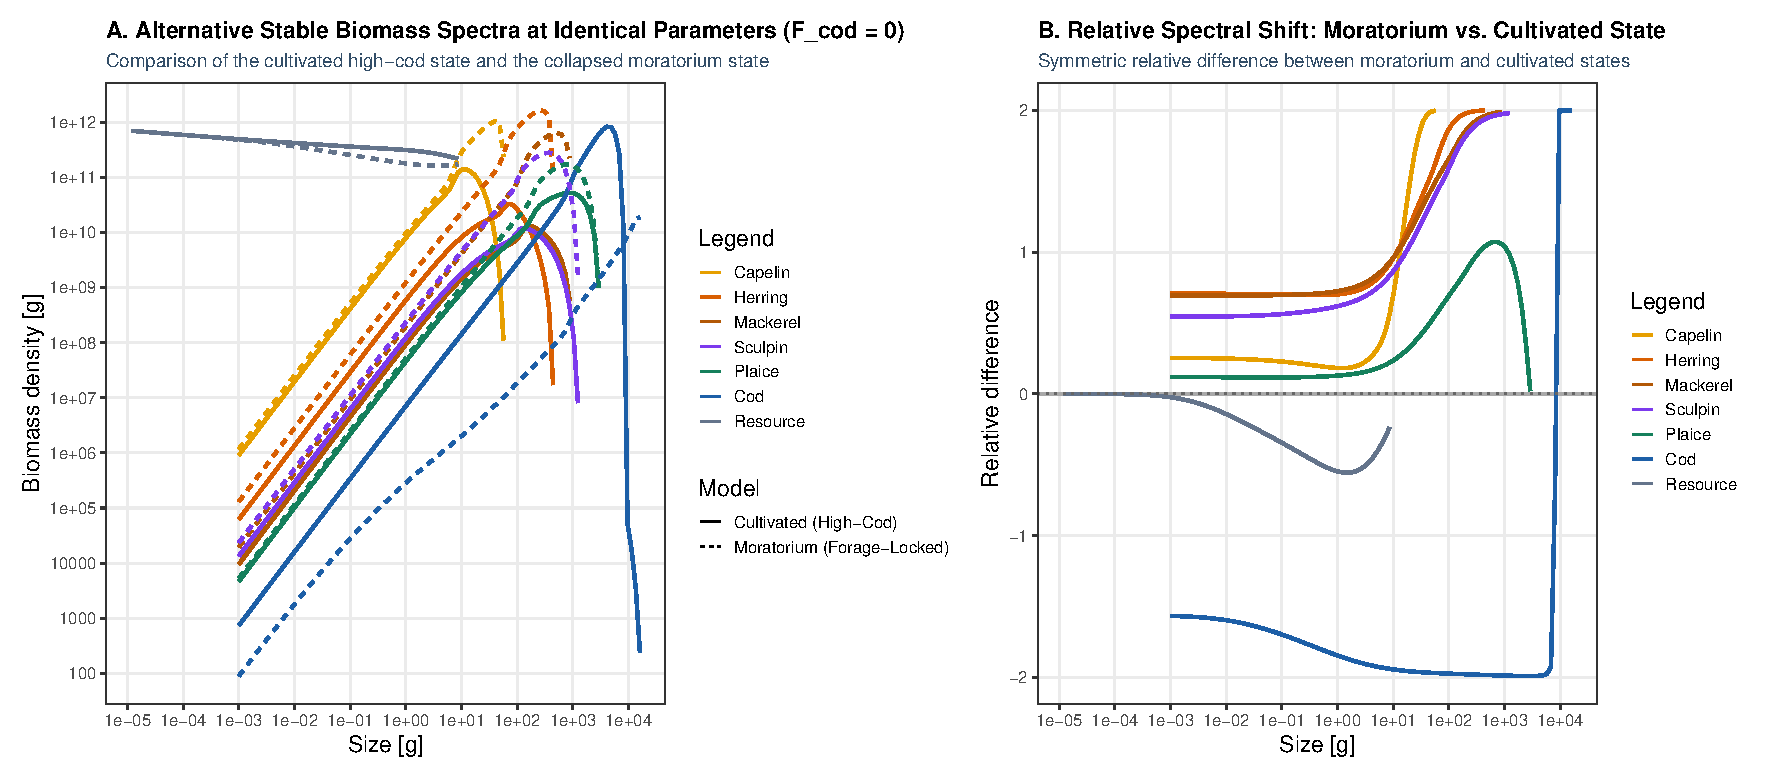
\includegraphics[width=0.98\textwidth]{figures/fig2_size_spectra_cascade.pdf}
  \caption{Alternative stable community size spectra at zero cod fishing ($F_{\mathrm{cod}} = 0\text{ yr}^{-1}$) under identical model parameters. \textbf{(A)} Biomass density per log-size bin $w^2 N(w)$ (\texttt{plotSpectra2}) comparing the cultivated high-cod state and the collapsed moratorium state alongside the plankton resource. \textbf{(B)} Symmetric relative spectral shift (\texttt{plotSpectraRelative}) illustrating the trophic cascade: severe truncation of the $0.1$--$15\text{ kg}$ cod spectrum coincides with an order-of-magnitude expansion of $5$--$900\text{ g}$ planktivores and sculpins and grazing depression of $0.01$--$10\text{ g}$ plankton.}
  \label{fig:spectra}
\end{figure}

Bisection along the state-space chord connecting the two attractors places the unstable saddle separatrix (the emergent Allee cultivation threshold) at $\mathrm{SSB}_{\mathrm{cod}} = 29.5\text{ kt}$ when $F_{\mathrm{cod}} = 0\text{ yr}^{-1}$, rising to $249.0\text{ kt}$ under moderate groundfish fishing ($F_{\mathrm{cod}} = 0.15\text{ yr}^{-1}$). Because the post-1992 stock ($5.7\text{ kt}$ in 1992; $10.2\text{ kt}$ in 2026) lies firmly below $29.5\text{ kt}$, offshore recruitment falls below replacement and only the $1.1\%$ inshore fjord refuge prevents total extirpation.

\subsection{Size-Structured Mechanism: The Dual Trophic Squeeze}

Decomposing size-specific vital rates between the two $F_{\mathrm{cod}} = 0$ attractors reveals why early-life cod survival collapses in the moratorium regime (Fig.~\ref{fig:mechanisms}). First, overabundant herring, mackerel, and capelin inflict intense ichthyoplankton and larval predation across $1\text{ mg}$--$1\text{ g}$, while benthic sculpins extend the gauntlet across $0.5$--$15\text{ g}$ settled $0$-group cod (Fig.~\ref{fig:mechanisms}A). Mean instantaneous predation mortality on cod across the $0.05$--$5\text{ g}$ nursery window rises from $0.25\text{ yr}^{-1}$ in the cultivated regime ($0.69\text{ yr}^{-1}$ in the historical fishery) to $7.33\text{ yr}^{-1}$ in the moratorium trap---a $29.7$-fold increase relative to the unexploited cultivated state and a $10.6$-fold increase relative to the historical sustainable fishery (Table~\ref{tab:equilibria}).

\begin{figure}[t!]
  \centering
  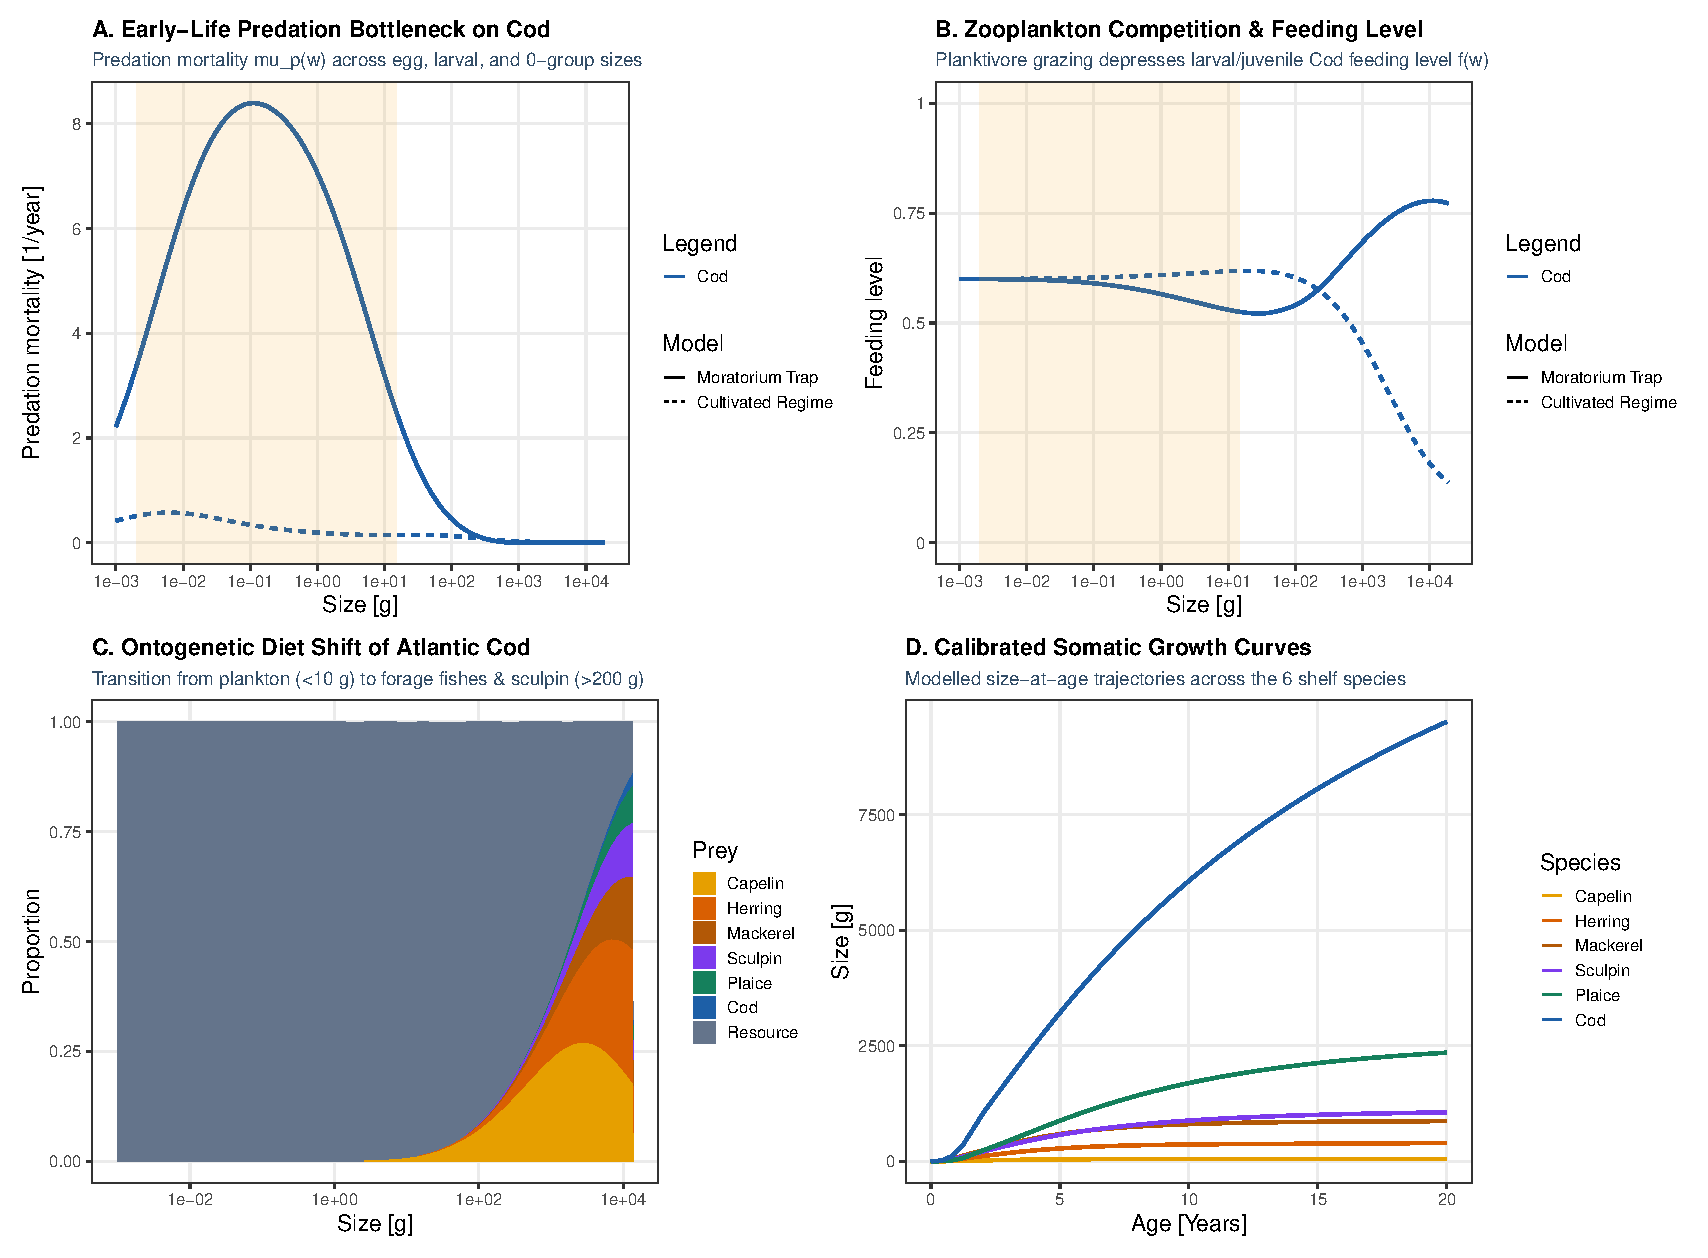
\includegraphics[width=0.90\textwidth]{figures/fig3_trophic_mechanisms.pdf}
  \caption{Size-structured bioenergetic and trophic mechanisms maintaining the moratorium trap. \textbf{(A)} Instantaneous predation mortality $\mu_p(w)$ on Atlantic cod across body mass (\texttt{plot2(getPredMort(...))}); shaded band highlights the vulnerable $2\text{ mg}$--$15\text{ g}$ egg, larval, and $0$-group window. \textbf{(B)} Cod feeding level $f(w)$ (\texttt{plot2(getFeedingLevel(...))}), showing zooplankton competition squeezing larval/juvenile intake while superabundant forage fish elevate feeding levels of surviving $>1\text{ kg}$ adult cod. \textbf{(C)} Ontogenetic diet composition of cod (\texttt{plotDiet}), shifting from plankton ($<10\text{ g}$) to capelin, clupeids, mackerel, and sculpins ($>200\text{ g}$). \textbf{(D)} Calibrated von Bertalanffy somatic growth trajectories across all six species (\texttt{plotGrowthCurves}).}
  \label{fig:mechanisms}
\end{figure}

Second, grazing by $>4600\text{ kt}$ of planktivores depletes the upper zooplankton spectrum ($0.01$--$10\text{ g}$; Fig.~\ref{fig:spectra}B), depressing feeding levels $f(w)$ of larval and small juvenile cod by 15\%--25\% inside the shaded nursery window (Fig.~\ref{fig:mechanisms}B). Slower somatic growth $g(w)$ compounds elevated $\mu_p(w)$ inside the survival integral of eq.~\eqref{eq:survival}. Paradoxically, the few cod that survive past $500\text{ g}$ and complete their ontogenetic shift onto piscivory (Fig.~\ref{fig:mechanisms}C) enjoy \emph{higher} adult feeding levels in the moratorium state than in the cultivated state (Fig.~\ref{fig:mechanisms}B) due to superabundant prey---explaining why healthy condition of rare large inshore cod can coexist with catastrophic recruitment failure at the population scale.

\subsection{Hysteresis Tipping Points and Ecosystem-Based Recovery Pathways}

Equilibrium continuation scans (\texttt{scanModel}) map out both the collapse hysteresis loop over directed cod fishing and the escape bifurcation over pelagic forage harvest (Fig.~\ref{fig:hysteresis}). Starting on the cultivated upper branch, increasing $F_{\mathrm{cod}}$ smoothly reduces equilibrium cod SSB from $1018.2\text{ kt}$ ($F_{\mathrm{cod}} = 0$) through $776.4\text{ kt}$ ($F_{\mathrm{cod}} = 0.15\text{ yr}^{-1}$) to $633.7\text{ kt}$ ($F_{\mathrm{cod}} = 0.225\text{ yr}^{-1}$), before crossing a sharp saddle-node collapse cliff at $F_{\mathrm{cod}}^{*} = 0.250\text{ yr}^{-1}$, where equilibrium cod SSB plummets to $0.75\text{ kt}$ (Fig.~\ref{fig:hysteresis}A). Reversing $F_{\mathrm{cod}}$ from $0.50\text{ yr}^{-1}$ all the way back to $0.00\text{ yr}^{-1}$ tracks the lower collapsed branch continuously without jumping back up, demonstrating mathematically why a zero-cod-fishing moratorium cannot exit the trap on its own.

\begin{figure}[t!]
  \centering
  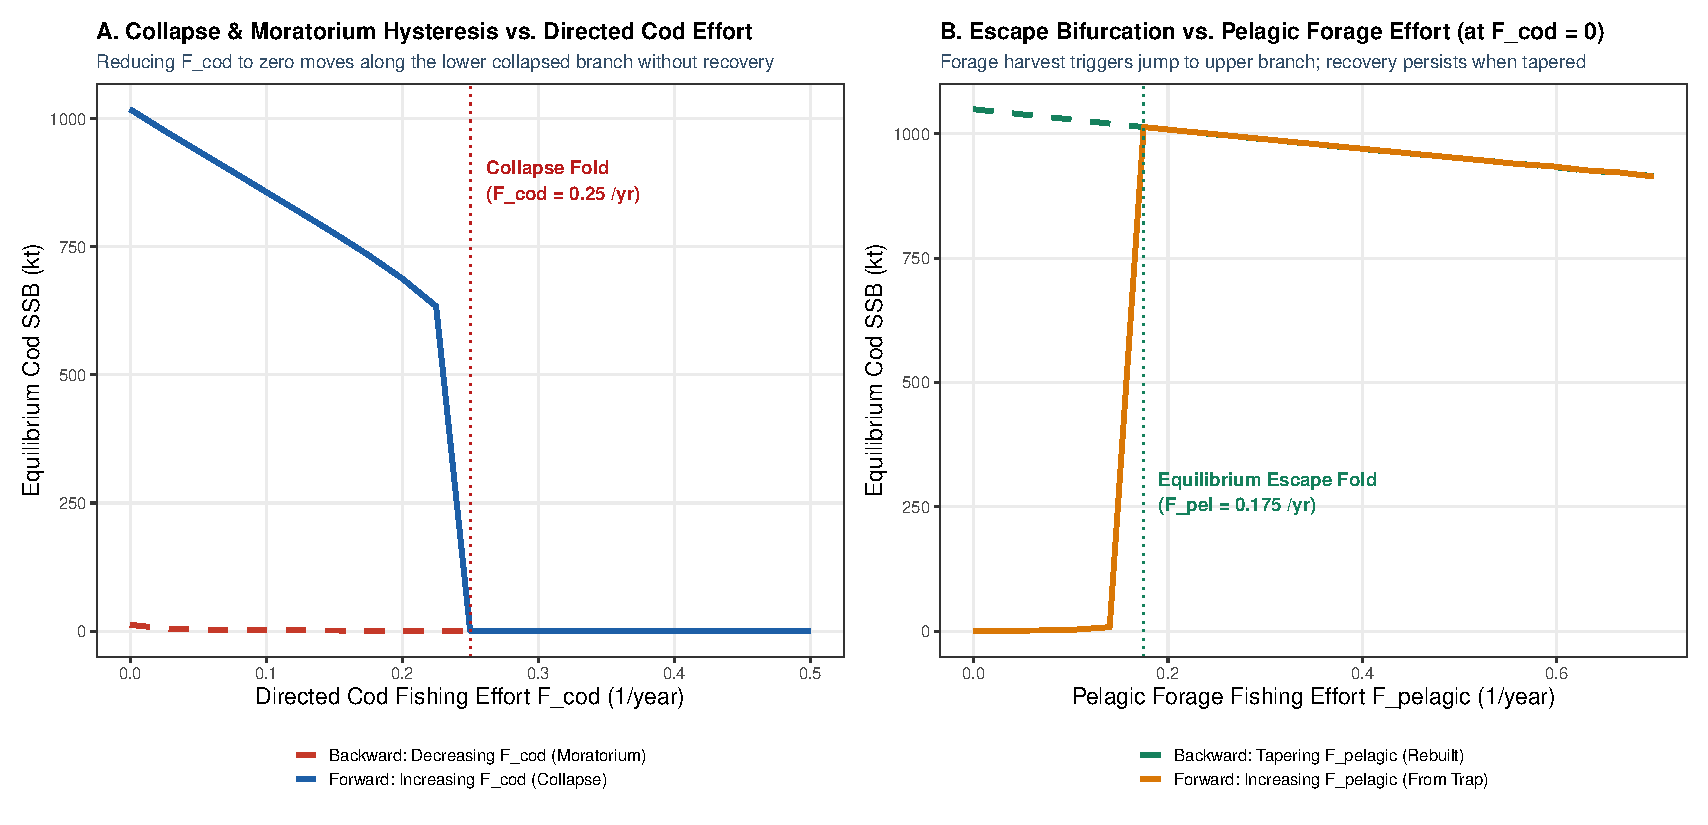
\includegraphics[width=0.98\textwidth]{figures/fig4_hysteresis_bifurcation.pdf}
  \caption{Equilibrium hysteresis and escape bifurcations computed via continuation (\texttt{scanModel}). \textbf{(A)} Equilibrium cod SSB versus directed cod trawl effort $F_{\mathrm{cod}}$: overfishing beyond the collapse fold ($F_{\mathrm{cod}}^{*} \approx 0.25\text{ yr}^{-1}$, solid blue) triggers irreversible collapse along the lower moratorium branch (dashed red) even when $F_{\mathrm{cod}}$ returns to zero. \textbf{(B)} Escape bifurcation versus pelagic forage fishing effort $F_{\mathrm{pelagic}}$ at $F_{\mathrm{cod}} = 0$: increasing $F_{\mathrm{pelagic}}$ from the moratorium state crosses an equilibrium escape fold at $F_{\mathrm{pelagic}}^{*} \approx 0.175\text{ yr}^{-1}$ (solid orange), jumping to the upper cultivated branch, which persists permanently when $F_{\mathrm{pelagic}}$ is tapered back to zero (dashed green).}
  \label{fig:hysteresis}
\end{figure}

Conversely, scanning pelagic forage effort $F_{\mathrm{pelagic}}$ upward from the collapsed state at $F_{\mathrm{cod}} = 0$ reveals an equilibrium escape fold at $F_{\mathrm{pelagic}}^{*} = 0.175\text{ yr}^{-1}$ (Fig.~\ref{fig:hysteresis}B)---remarkably close to, yet strictly above, the $0.15\text{ yr}^{-1}$ baseline pelagic exploitation rate (which accounts for the slow $-0.0084\text{ yr}^{-1}$ eigenvalue at the moratorium attractor). Once $F_{\mathrm{pelagic}}$ pushes the community onto the upper branch, tapering $F_{\mathrm{pelagic}}$ downward from $0.70\text{ yr}^{-1}$ back to $0.15\text{ yr}^{-1}$ (or $0.00\text{ yr}^{-1}$) tracks the upper cultivated branch ($\mathrm{SSB}_{\mathrm{cod}} > 910\text{ kt}$), proving that trophic-release harvest need only be \emph{transitional} rather than permanent.

Crucially, however, dynamic 40-year policy projections from 2026 to 2066 highlight the difference between asymptotic century-scale bifurcations and management-relevant recovery horizons (Fig.~\ref{fig:scenarios}; Table~\ref{tab:policies}). Near $F_{\mathrm{pelagic}} \approx 0.20$--$0.35\text{ yr}^{-1}$, critical slowing down in the ``ghost'' of the saddle-node bottleneck delays rebuilding beyond 60--100 years. Across our six policy strategies (Table~\ref{tab:policies}):
\begin{itemize}
  \item \textbf{Strategy 1 (Status Quo Moratorium, $F_{\mathrm{pel}}=0.15, F_{\mathrm{meso}}=0.05, F_{\mathrm{cod}}=0$):} Cod remains trapped at $12.0\text{ kt}$ SSB in 2066 ($1.5\%$ of pre-collapse SSB; Fig.~\ref{fig:scenarios}A).
  \item \textbf{Strategy 2 (Premature Cod Reopening, $F_{\mathrm{cod}} \to 0.25\text{ yr}^{-1}$ in 2046):} Reopening cod trawling without prior trophic release drives remnant cod SSB down to $0.9\text{ kt}$.
  \item \textbf{Strategy 3 (Sculpin Mesopredator Harvest Only, $F_{\mathrm{meso}}=0.45\text{ yr}^{-1}$):} Thinning benthic sculpins alone yields slow partial release ($\mathrm{SSB}_{\mathrm{cod}} = 34.1\text{ kt}$ by 2066), because unthinned clupeids and mackerel continue inflicting heavy pelagic egg/larval mortality.
  \item \textbf{Strategy 4 (Pelagic Forage Harvest, $F_{\mathrm{pel}}=0.55\text{ yr}^{-1}, F_{\mathrm{cod}}=0$):} Selective midwater/purse-seine harvest of abundant herring, mackerel, and capelin slashes larval cod mortality, crosses the cultivation threshold within $\sim 16$ years, and rebuilds cod SSB to $958.5\text{ kt}$ by 2066 ($123\%$ of pre-collapse fishery SSB; Fig.~\ref{fig:scenarios}B).
  \item \textbf{Strategy 5 (Combined Sustained Harvest, $F_{\mathrm{pel}}=0.55, F_{\mathrm{meso}}=0.35, F_{\mathrm{cod}}=0$):} Synergistic pelagic and benthic release produces the fastest unfished recovery ($\mathrm{SSB}_{\mathrm{cod}} = 985.1\text{ kt}$), though sustained heavy forage harvest after adult cod already resumes predation unnecessarily depresses equilibrium forage yield ($91.8\text{ kt}\cdot\text{yr}^{-1}$).
  \item \textbf{Strategy 6 (Adaptive 20-Year Pulse + Taper \& Reopened Cod Fishery):} Applying $F_{\mathrm{pel}} = 0.65\text{ yr}^{-1}$ and $F_{\mathrm{meso}} = 0.45\text{ yr}^{-1}$ during 2026--2046 drives cod SSB well past the $249.0\text{ kt}$ fishery separatrix, allowing pelagic and mesopredator effort to taper back to baseline ($0.15$ and $0.05\text{ yr}^{-1}$) in 2046 while reopening a sustainable size-selective cod fishery ($F_{\mathrm{cod}} = 0.15\text{ yr}^{-1}$; Fig.~\ref{fig:scenarios}C,D). By 2066, cod SSB reaches $475.3\text{ kt}$ (continuing upward toward its $776.3\text{ kt}$ equilibrium) while delivering $369.4\text{ kt}\cdot\text{yr}^{-1}$ of balanced, high-value multispecies yield.
\end{itemize}

\begin{figure}[t!]
  \centering
  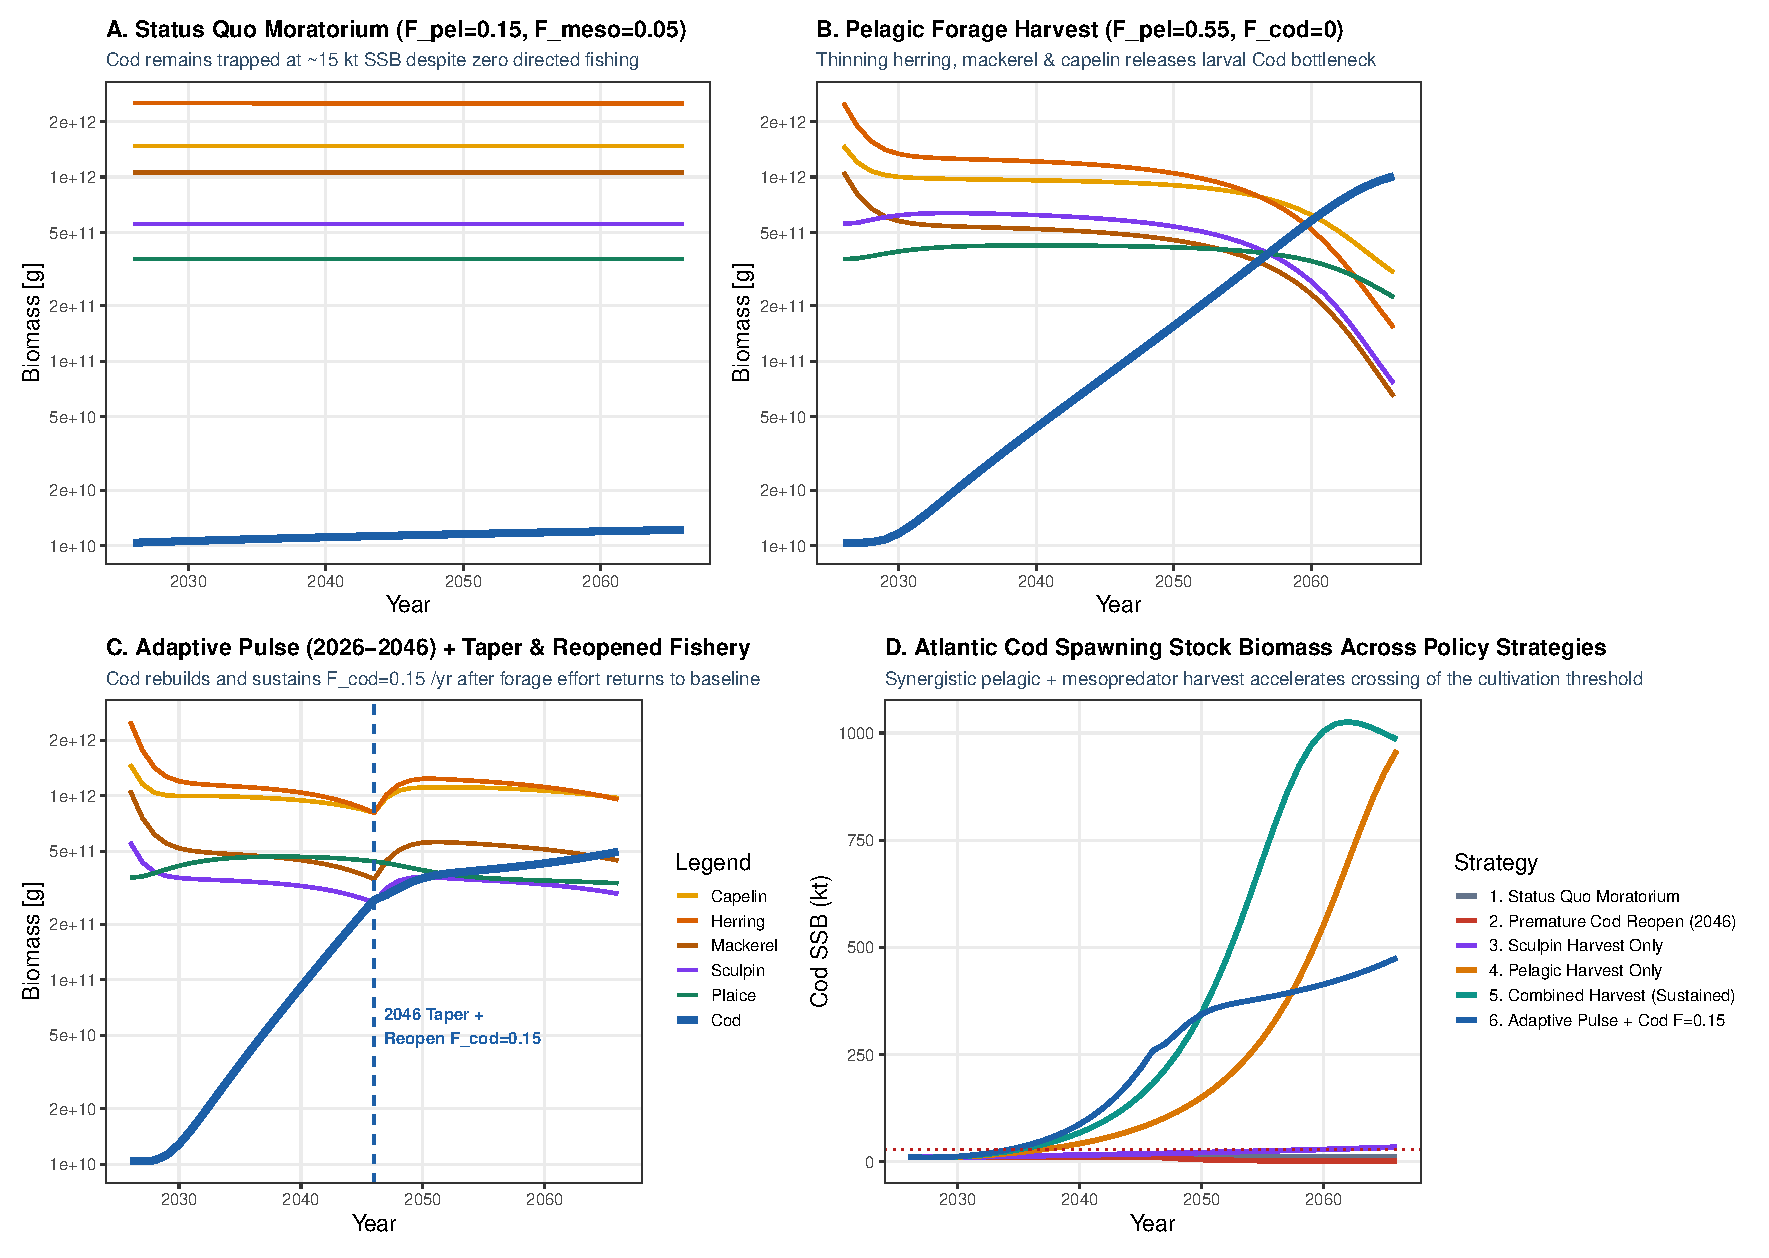
\includegraphics[width=0.90\textwidth]{figures/fig5_recovery_strategies.pdf}
  \caption{Projected 40-year ecosystem recovery trajectories (2026--2066) across management strategies. \textbf{(A)} Status quo moratorium leaves cod suppressed beneath abundant planktivores and sculpins. \textbf{(B)} Pelagic forage harvest ($F_{\mathrm{pel}} = 0.55\text{ yr}^{-1}$) triggers trophic cascade reversal and full cod rebuilding. \textbf{(C)} Adaptive two-phase pulse ($F_{\mathrm{pel}} = 0.65, F_{\mathrm{meso}} = 0.45\text{ yr}^{-1}$ during 2026--2046), followed in 2046 by tapering forage/sculpin effort back to baseline and reopening directed cod fishing ($F_{\mathrm{cod}} = 0.15\text{ yr}^{-1}$). \textbf{(D)} Comparison of cod SSB trajectories across all six policy strategies relative to the $F_{\mathrm{cod}} = 0$ cultivation separatrix (dotted red line).}
  \label{fig:scenarios}
\end{figure}

\begin{table}[t!]
\centering
\caption{Comparison of 40-year management scenarios (2026--2066) initialized from the 2026 moratorium state ($\mathrm{SSB}_{\mathrm{cod}} = 10.2\text{ kt}$). Arrows ($\to$) denote adaptive Phase-II rate transitions in year 2046.}
\label{tab:policies}
\vspace{0.4em}
\resizebox{\textwidth}{!}{%
\begin{tabular}{lrrrrc}
\hline
Policy Scenario & $F_{\mathrm{cod}}$ ($\text{yr}^{-1}$) & $F_{\mathrm{pelagic}}$ ($\text{yr}^{-1}$) & $F_{\mathrm{mesopred}}$ ($\text{yr}^{-1}$) & 2066 Cod SSB (kt) & 2066 Total Yield ($\text{kt}\cdot\text{yr}^{-1}$) \\
\hline
1. Status Quo Moratorium        & $0.00$         & $0.15$         & $0.05$         &  12.0 (2\%)   & 663.1 \\
2. Premature Cod Reopening      & $0.00 \to 0.25$& $0.15$         & $0.05$         &   0.9 (0.1\%) & 671.1 \\
3. Sculpin Harvest Only         & $0.00$         & $0.15$         & $0.45$         &  34.1 (4\%)   & 757.7 \\
4. Pelagic Forage Harvest       & $0.00$         & $0.55$         & $0.05$         & 958.5 (123\%) & 172.3 \\
5. Combined Harvest (Sustained) & $0.00$         & $0.55$         & $0.35$         & 985.1 (127\%) &  91.8 \\
6. Adaptive Pulse + Cod Fishery & $0.00 \to 0.15$& $0.65 \to 0.15$& $0.45 \to 0.05$& 475.3 (61\%)$^{\dagger}$ & 369.4 \\
\hline
\multicolumn{6}{l}{\footnotesize $^{\dagger}$Monotonically approaching the self-sustaining $776.3\text{ kt}$ cultivated fishery equilibrium after 2046 reopening.}
\end{tabular}%
}
\end{table}

Mapping the full two-dimensional Phase-I effort surface $(F_{\mathrm{pelagic}}, F_{\mathrm{mesopred}})$ under the adaptive taper protocol with reopened $F_{\mathrm{cod}} = 0.15\text{ yr}^{-1}$ (Fig.~\ref{fig:surface}) reveals a clear synergistic frontier: while neither $F_{\mathrm{pelagic}} \le 0.35\text{ yr}^{-1}$ nor $F_{\mathrm{mesopred}}$ alone crosses the $249.0\text{ kt}$ reopened-fishery separatrix within 20 years, combining $F_{\mathrm{pelagic}} \in [0.65, 0.80]\text{ yr}^{-1}$ with $F_{\mathrm{mesopred}} \in [0.35, 0.60]\text{ yr}^{-1}$ (or $F_{\mathrm{pelagic}} = 0.55\text{ yr}^{-1}$ with $F_{\mathrm{mesopred}} = 0.60\text{ yr}^{-1}$) reliably drives 2066 cod SSB across $264$--$780\text{ kt}$ while sustaining $214$--$490\text{ kt}\cdot\text{yr}^{-1}$ of diversified post-taper landings.

\begin{figure}[t!]
  \centering
  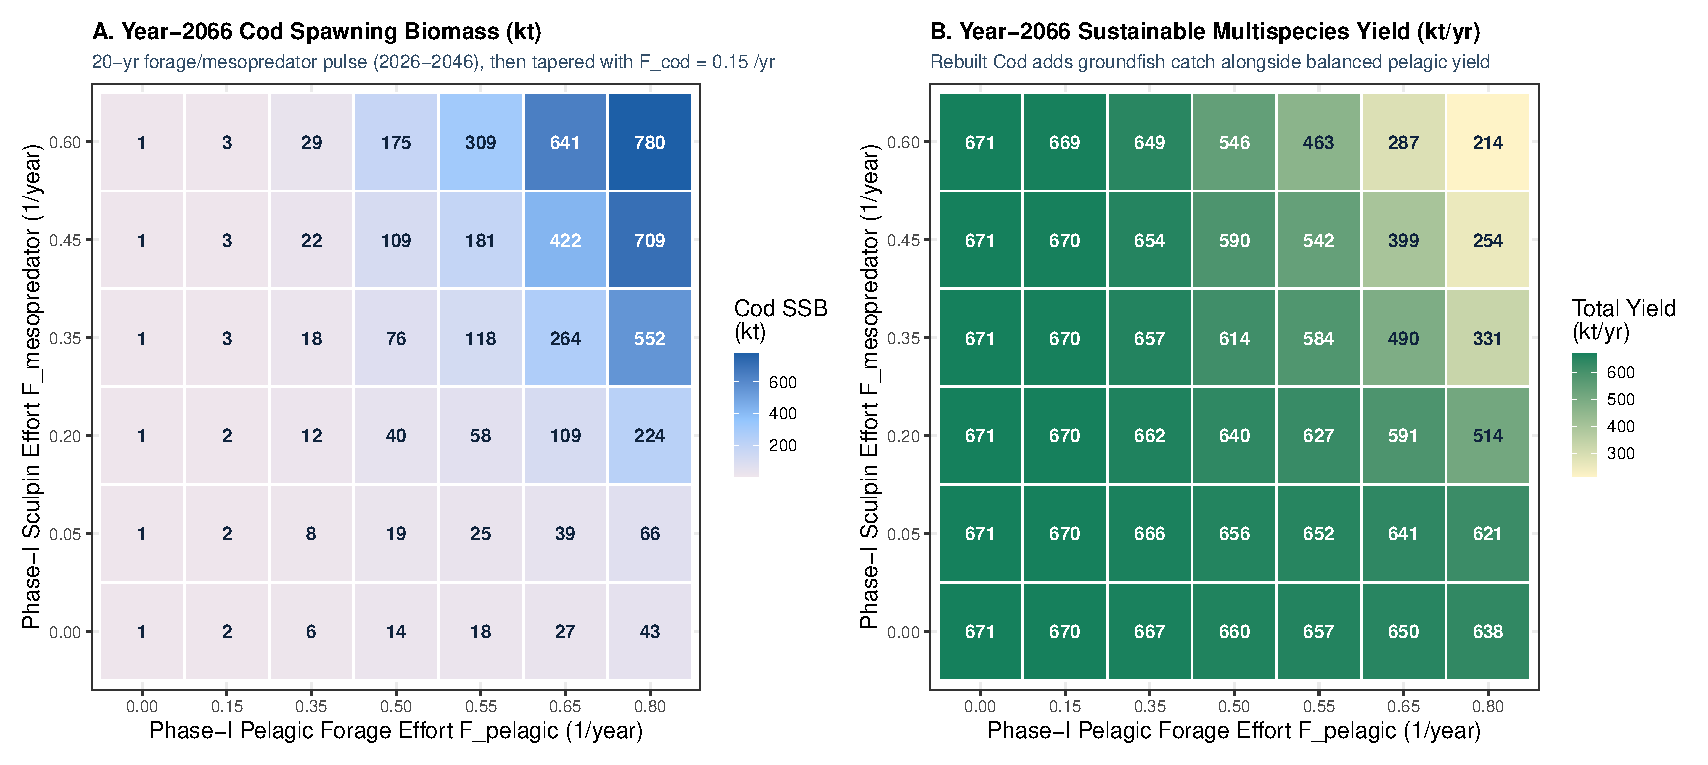
\includegraphics[width=0.98\textwidth]{figures/fig6_policy_tradeoffs.pdf}
  \caption{Two-dimensional policy response surface across Phase-I (2026--2046) pelagic forage effort $F_{\mathrm{pelagic}}$ and sculpin mesopredator effort $F_{\mathrm{mesopred}}$, evaluated in year 2066 after tapering both fleets back to baseline ($0.15$ and $0.05\text{ yr}^{-1}$) and reopening directed cod fishing at $F_{\mathrm{cod}} = 0.15\text{ yr}^{-1}$ in 2046. \textbf{(A)} Year-2066 cod SSB (kt), showing the sharp recovery separatrix frontier. \textbf{(B)} Year-2066 sustainable multispecies yield ($\text{kt}\cdot\text{yr}^{-1}$).}
  \label{fig:surface}
\end{figure}

\section{Discussion}

\subsection{Why Single-Species Moratoria Fail Under Ontogenetic Symmetry Breaking}

Our results provide a mechanistic, physiologically structured resolution to the 34-year Northwest Atlantic cod moratorium paradox. Standard single-species fisheries theory assumes that per-capita recruitment rate increases monotonically as spawner biomass declines, guaranteeing a unique globally attracting unexploited equilibrium once $F = 0$. In size-structured marine food webs, however, apex demersal piscivores begin life at $1\text{ mg}$---four orders of magnitude smaller than the adult forage fishes they eventually consume \citep{walters2001cultivation,andersen2019fish}. Our size-spectrum model demonstrates that this ontogenetic symmetry breaking generates true multi-species bistability at $F_{\mathrm{cod}} = 0$ without invoking exogenous regime shifts in ocean climate or unmodelled adult mortality. Once historical trawl overfishing pushed cod below the cultivation threshold, predation release allowed herring, mackerel, capelin, and sculpins to expand more than five-fold \citep{frank2005trophic}, inflating nursery predation mortality on $0.05$--$5\text{ g}$ cod nearly thirty-fold relative to the unexploited cultivated state and trapping remnant cod in coastal fjord refuges \citep{lilly2013review}.

Furthermore, our eigenvalue and continuation analyses expose a crucial distinction between \emph{equilibrium} tipping points and \emph{operational} rebuilding timescales. Although the collapsed branch terminates at an equilibrium pelagic harvest fold near $F_{\mathrm{pelagic}}^{*} \approx 0.175\text{ yr}^{-1}$ (just above the $0.15\text{ yr}^{-1}$ status quo), trajectories at $F_{\mathrm{pelagic}} = 0.20$--$0.35\text{ yr}^{-1}$ linger for generations inside the saddle-node bottleneck's slow manifold. This explains why modest fluctuations in pelagic landings or transient forage declines \citep{frank2011transient} have produced hesitant, reversible pulses of juvenile cod rather than decisive shelf-wide recovery.

\subsection{Ecological Guardrails, Capelin Conservation, and Gear Selectivity}

Proposing increased harvest on forage fishes and mesopredators to catalyze apex groundfish recovery requires careful ecological qualification and strict operational guardrails \citep{pikitch2012little,garcia2012reconsidering}. In the Northwest Atlantic---particularly NAFO Divisions 2J3KL off Newfoundland and Labrador---capelin is a foundational forage species supporting breeding seabirds, humpback whales, harp seals, and adult cod growth and fecundity \citep{rose2002capelin,lilly2013review}. Three findings from our size-spectrum analysis directly inform precautionary implementation:

First, \emph{selective targeting of temperate ichthyoplankton predators outperforms indiscriminate capelin depletion}. In our interaction structure and in empirical Gulf and Scotian Shelf time series \citep{swain2000pelagic}, adult herring and mackerel exert the strongest per-capita predation on pelagic cod eggs and larvae during spring--summer spawning overlap, whereas benthic sculpins ambush newly settled $0$-group cod in coastal nurseries. Concentrating Phase-I harvest quotas on abundant herring and mackerel complexes during seasonal overlap, paired with localized sculpin pot/trap removals in priority cod nursery bays, achieves trophic release while safeguarding capelin biomass above precautionary forage thresholds (e.g., $\ge 40\%$ of unexploited carrying capacity; \citealt{pikitch2012little}).

Second, \emph{trophic-release harvest must be adaptive and temporary, never permanent}. As demonstrated by Strategy~5 versus Strategy~6 (Table~\ref{tab:policies}; Fig.~\ref{fig:scenarios}C), maintaining high pelagic fishing mortality after adult cod has crossed the cultivation separatrix subjects forage stocks to simultaneous top-down predation and heavy fishing, eroding total ecosystem yield. Instead, harvest control rules should tie pelagic quotas inversely to surveyed $0$-group cod survival and adult cod biomass: as rebuilding cod naturally resumes top-down forage control in years 12--20, pelagic and mesopredator effort steps back down to baseline.

Third, \emph{gear selectivity must strictly prevent juvenile and adult cod bycatch}. Rebuilding fails immediately if expanded forage or mesopredator fisheries inflict incidental mortality exceeding $F_{\mathrm{cod}} \approx 0.05\text{ yr}^{-1}$ during Phase~I. Acoustic-targeted midwater pelagic trawls, purse seines, and shallow-water sculpin traps achieve high species and size selectivity with minimal demersal cod contact, and reopened Phase-III cod fisheries should maintain large mesh/hook selectivity ($L_{50} \ge 52\text{ cm}$) and conservative target mortality ($F_{\mathrm{cod}} \approx 0.15\text{ yr}^{-1}$, well below the $0.25\text{ yr}^{-1}$ hysteresis cliff).

\subsection{Interactive Decision-Support Tool and Future Extensions}

Because nonlinear hysteresis, saddle-node thresholds, and multi-fleet trade-offs are counter-intuitive when communicated solely through static equations, we developed an open-access interactive policy explorer (\texttt{docs/index.html}) coupled directly to precomputed \texttt{mizer} simulation grids. Policy makers can manipulate pelagic, mesopredator, and post-rebuild cod fishing mortalities, toggle adaptive Phase-II tapering, and inspect real-time responses in cod SSB, guild biomasses, fleet yields, size spectra, and early-life predation mortality. Future extensions of this work should incorporate spatial metapopulation connectivity between inshore Newfoundland fjords and offshore banks, seasonal ocean warming impacts on metabolic maintenance ($k_{s,i}$) and plankton size structure ($\lambda$), and explicit pinniped predation dynamics to tailor division-specific rebuilding plans across NAFO subareas.

\section{Conclusions}

Three decades of commercial cod moratoria in the Northwest Atlantic demonstrated that halting directed fishing on a collapsed apex piscivore is necessary---but not sufficient---when ontogenetic role reversal locks the community into an alternative forage- and mesopredator-dominated stable state. Using a calibrated multi-species size-spectrum model in \texttt{mizer}, we proved that identical biological parameters support both a cultivated high-cod equilibrium ($1018.2\text{ kt}$ SSB) and an asymptotically stable collapsed moratorium equilibrium ($15.8\text{ kt}$ SSB) maintained by a thirty-fold surge in early-life cod predation mortality and juvenile food competition. Breaking this moratorium trap requires managing the size spectrum as an interconnected food web: a time-limited, selective harvest pulse on overabundant pelagic planktivores and benthic sculpins releases the juvenile cod bottleneck, crosses the cultivation threshold within two decades, and restores a productive, self-sustaining Northwest Atlantic cod fishery.

\section*{Data and Code Availability}

All R scripts required to build and calibrate the \texttt{mizer} model (\texttt{R/00\_\allowbreak model\_\allowbreak functions.R}, \texttt{R/01\_\allowbreak build\_\allowbreak and\_\allowbreak calibrate\_\allowbreak model.R}), reproduce the Jacobian stability, continuation, and scenario analyses (\texttt{R/02\_\allowbreak analyse\_\allowbreak bistability\_\allowbreak and\_\allowbreak scenarios.R}), generate all manuscript figures and web simulation data (\texttt{R/03\_\allowbreak generate\_\allowbreak figures\_\allowbreak and\_\allowbreak web\_\allowbreak data.R}), saved \texttt{MizerParams} objects (\texttt{models/}), and the self-contained interactive policy web application (\texttt{docs/}) are included in this repository.

\bibliographystyle{apalike}
\bibliography{references}

\end{document}
